\documentclass[11pt]{article}
\usepackage[T1]{fontenc}
\usepackage[latin1]{inputenc}
\usepackage{enumerate}
\usepackage{setspace}
\usepackage{amsmath,amssymb,amsthm}
\usepackage{graphicx}
\usepackage{bbm}
\usepackage[round]{natbib}
\usepackage[nohead]{geometry}
\usepackage[bottom]{footmisc}
\usepackage{indentfirst}
\usepackage{endnotes}
\usepackage{graphicx}%
\usepackage{eurosym}
\usepackage{array}
\usepackage{booktabs}
\usepackage{caption}
\usepackage{subcaption}
% \usepackage[hidelinks]{hyperref}
\usepackage{floatrow} %[capposition=top]
\floatsetup{footposition=bottom,capposition=top}
\renewcommand{\labelitemi}{--}
\renewcommand{\labelitemii}{$\bullet$}
\bibliographystyle{chicago}
% \geometry{left=1in,right=1in,top=1.00in,bottom=1.0in}
\let\olditemize\itemize
\renewcommand{\itemize}{
  \olditemize
  \setlength{\itemsep}{-1pt}
}

\begin{document}

\title{Price dispersion on the French retail gasoline market\ \\ \ \\(Very preliminary)}
\author{Etienne Chamayou\thanks{e-mail:
\textit{etienne.chamayou@ensae.fr}}\medskip\\{\normalsize CREST and Department of Economics, Ecole Polytechnique }}
\maketitle

\sloppy%

\onehalfspacing

\textbf{Abstract:}
This paper studies static and dynamic price dispersion in the French retail gasoline market. Using a large panel of daily gas station prices to produce statistics accounting for local competition, it finds support for a link between consumer information and price dispersion. Indeed, among competitors exhibiting similar price levels, changes in price rankings are found to be positively correlated with the distance separating both sellers, namely with the difficulty for consumers to compare prices. Supermarkets, which generally operate at low markups, are over-represented among pairs of competitors with similar price levels as well as among pairs of competitors which regularly set at the very same price. This is consistent with them addressing demand from well informed price sensitive customers, as opposed to oil company and independent gas stations generally more focused on less informed and/or more loyal or captive customers.

\strut

\textbf{Keywords:} Consumer search, Price dispersion

\strut

\textbf{JEL Classification Numbers:} L13

\pagebreak%
%\doublespacing

\section{Introduction}

The seminal paper of the consumer search literature, \cite{STI61}, draws attention to the relation between the "ignorance in the market", namely consumers' lack of information, and price dispersion i.e. the persistence over time of different prices for a homogeneous good. While the paper only provides evidence of static price dispersion e.g. retailers posting different prices for a given car model in a suburb, thus leaving room for unobserved differentiation, the empirical literature would soon make the case stronger through the observation of price dynamics. The ranking of sellers in price distributions would indeed be observed to vary significantly over time, making it difficult for consumers to find the cheapest price.

The retail gasoline market offers interesting case studies for empirical industrial organization. Indeed, consumers generally buy only one product which is essentially homogeneous, suggesting a potentially tough price competition whenever the density of sellers is high enough. More generally, transportation costs can be expected to relax competition, as well as uncertainty about prices, all the more as oil cost variations generate constant retail price variations.

Competition in the retail gasoline market has attracted a lot of attention in France over last years. In 2006, a price comparison website was launched by the Ministry of Economics with a view to increase transparency in the market. In 2011, a large inquiry was ordered by the government as retail price adjustments to oil cost variations were suspected to occur faster upwards than downwards (the "Rocket and feathers" hypothesis first investigated by \cite{BAC91} in the UK). Little evidence was yet found and the report rather emphasized signs pointing toward a significant degree of competitiveness. More recently, in August 2012, following an election promise, the governement of the then newly elected French President Francois Hollande implemented a 3 Euro cents per litre tax cut during 3 months, asking gasoline retailers on the market to produce a similar effort. The French retail gasoline market thus tends to be thoroughly scrutinized.

More generally, in a context where dynamic prices generate heightened debates (e.g. Amazon), the idea to monitor competition by constraining firms to increase transparency enjoys strong popularity among politicians. Nevertheless, economic theory shows that measures affecting information can have adverse effects. Costless monitoring indeed makes collusion easier, while aligned prices provide little incentive for consumers to become or remain informed.

The following paper elaborates on the methodology used by \cite{TAP11} to study price dispersion, in order to deal with the differentiation observed in the French market and discuss the sources of observed price dispersion. Among pairs of competing stations exhibiting little differentiation, price dispersion is found to significantly increase with distance separating stations (very close competitors vs. competitors located further away), providing support for the connection between consumer information and price dispersion. The effect is significantly weaker for differentiated competitors. At the market level, price dispersion is found to increase with the number of competitors and decrease with price level.

\section{Literature}

A major contribution of the consumer search literature was made by \cite{VAR80} through the modeling of price dispersion as a result of mixed pricing strategies. According to the paper, price dispersion thereby obtained could be interpreted as "temporal" price dispersion, typically in the form of "sales". This provided a rationale for rank reversals i.e. a seller being cheaper or more expensive than a competitor with positive probabilities.

The dynamic interpretation of the model is not unambiguous however. In the model, firms are ex-ante indifferent between all prices in the support of the equilibrium price distribution (also holds in terms of randomization over utilities). Ex-post, indifference obviously no more exists. The cheapest firm attracts shoppers but would be better off increasing its price to match the second cheapest price. Other firms would rather increase their price to consumers' reservation price, or try to undercut the cheapest firm. In the retail gasoline market, while it may not be possible for firms to change prices on too frequent a basis, periods of significant oil price variations reveal that gas stations can adjust prices on a daily basis. If one admits that gas stations play according to \cite{VAR80} on a given day, it is thus not clear why sellers would wish to keep prices unchanged the following day. A possible explanation may be that firms refrain from changing prices too often for fear of triggering more search by consumers and thus more intense competition. Whether this can be obtained in a fully competitive setting  or would require some kind of collusion (possibly at the retail chain level or at the local level) remains an open question.

\cite{TAP11} work with a data set including daily prices of gas stations within four states in the US over one year and a half. They argue that gas stations located across the same corner should display less rank reversal vs. those a bit further, since consumer information on prices should decrease with distance. This is shown to be true and all the more convincing as close gas stations display a lower average spread. Regressions of various measures accounting for price dispersion on marginal costs and the number of firms in the market (built by considering circles of varying radiuses) yields results consistent with the extension of \cite{VAR80} proposed by the paper (resp. negative and positive impacts). All the analysis is performed with raw prices, which, I argue, is bound to bias some results.

\section{The French retail gasoline market}

\subsection{Data sources}

Since 2007, French gasoline retailers are required by law to keep prices updated on the price comparison website prix-carburants.gouv.fr. Small gas stations%
\footnote{Stations having sold over 500m$^{3}$ gas the previous year%
} are exempted from this obligation hence c.10,000 gas stations are observed out of an estimated total number of 12,000 retailers%
\footnote{A 2012 governmental report on the French retail gasoline market notes that "nobody knows precisely the number of gas stations operating in the markets". Two other comparison websites, carbeo.com and zagaz.com, were created in 2005 and 2006, relying on user provided information. Zagaz has stuck to its "crowdsourcing" philosophy until 2014, while Carbeo started purchasing licences from the government in 2009. In 2012, the governmental body in charge of town and country planning worked with Zagaz data to study the French retail gas station network.%
}. For this study, prices and brand changes were collected from the website on a daily basis between September 4, 2011 and December 4, 2014, hence a period of about 3 years, interrupted by some gaps related to data acquisition issues. Highway gas stations are excluded for the core of the analysis. Additionally, price series of XXX were deemed to be unreliable based on value and rigidity criteria, leading to their exclusion. Station locations, including gps coordinates, and characteristics were collected several times over the period in order to cover new retailer registrations, and potential changes in station amenities. Information on station location was checked and improved in several steps (cf. appendix), and local market characteristics were associated to stations based on municipalities or relevant larger areas.

\subsection{Retail gasoline distribution}

The size of the French gas station network has been decreasing at a steady pace over the last decades, from c. 40,000 in 1980 to c. 12,000 currently.  Unlike most other European countries, the French market is characterized by a strong competitive pressure generated from gas stations operated by supermarket chains. They currently represent c. 50\% of sales in retail gasoline.

As of May 20, 2014, Zagaz listed c. 12,832 gas stations, but no price was recorded over the last months/years for many of them so that this figure most likely overestimates the actual number of gas stations. In April 2013, UFIP quoted the numbers of 11,662 (4,947 supermarkets and 6,715 "traditional" players) for 2012 and 11,476 for 2013 (4,979 supermarkets and 6,497 "traditional" players, source: Nielsen). UFIP also reported that 1,506 gas stations sold less than 500m$^{3}$ in 2012 (1,433 in 2013), with the median gas station selling between 1,000 and 3,000m$^{3}$ (same for 2013).

Gas stations are essentially either owned and operated by a chain or with a "location-gerance" contract according to which the manager receives a commission on gasoline sold (e.g. only 200 gas stations set prices independently among gas stations from Total brand). There is significant evidence that many gas stations hardly make any profits: oil companies exiting the market (Shell and BP), drastically reducing the size of their organic network (Esso), bankrupts or terminations of independent gas stations etc.

Key cost components are the cost of wholesale gasoline, including delivery fees,  gas station operating expenses, and taxes. Taxes included a fix part called TICPE, which slightly varies between regions, and the classical Value-Added Tax (19.6\% over the period studied, which bear on cost and TICPE).

Diesel consumption currenlty accounts for c. 80\% of total gasoline consumption. A signicant increase in the diesel share was achieved over the last decades through a lower tax on diesel. At a very aggregate level, two kinds of consumers can be distinguished: businesses and individual customers. Businesses are typically offered card programs which allow them to monitor employees' consumptions and obtain rebates. An important implication is that the price of the gas station is irrelevant (or only partly relevant) to a significant number of transations in the market.
Consumers can get information about prices from a variety of sources: at gas stations, on their gps, on mobile phone applications (e.g. Zagaz, Carbeo, Essence Free) and on a computer or mobile phone browser (Prix-Carburants.gouv.fr).

\subsection{Context of studied period}

The period covered is marked by two significant events of different natures. One is a change of pricing strategy by a leading retail brand affecting the whole country and the other is a governmental intervention.

The first event is the progressive conversion by the oil company "Total" of c. 600 of its gas stations to low cost gas stations branded "Total Access" i.e. gas stations whose prices are aligned with supermarket gas stations. About half the conversions occur during the period covered by the paper. Though these conversions are obviously not heterogeneous shocks to the market, they yet involve a significant number of gas stations lowering their price by c. 10 Euro cents per liter virtually overnight.

The second event is of political nature. On August 29, 2012, a decrease in price of 6 Euro cents per litre was announced by the government, following an election promise made by Francois Hollande. This decrease was (to be) achieved by a decrease of tax of 3 Euro cents per litre and an equivalent "effort" by gas station operators. Also, it must be noted that a small portion of the tax on gasoline is set by regions on an annual basis.

\subsection{Descriptive statistics}

\subsubsection{Retail price vs. wholesale cost of diesel}

Descriptive statistics are provided for a period of 640 days starting September 9, 2011 and ending May 6, 2013. Four subperiods of data are yet missing for various technical reasons, thus reducing the number of observed days to 564\footnote{Respective day lengths of missing subperiods are 11 (2012/07/08-2012/07/18), 10 (2012/08/13-2012/08/22), 49 (2012/12/04-2013/01/21) and 6 (2013/04/04-2013/04/09).}. The end of the period studied has been determined arbitrarily to avoid including another missing subperiod and to keep the database to a reasonable size.

\begin{figure}[!h]
    \caption{Diesel prices and retail gross margin (09/2011-06/2013)}
	\centering
		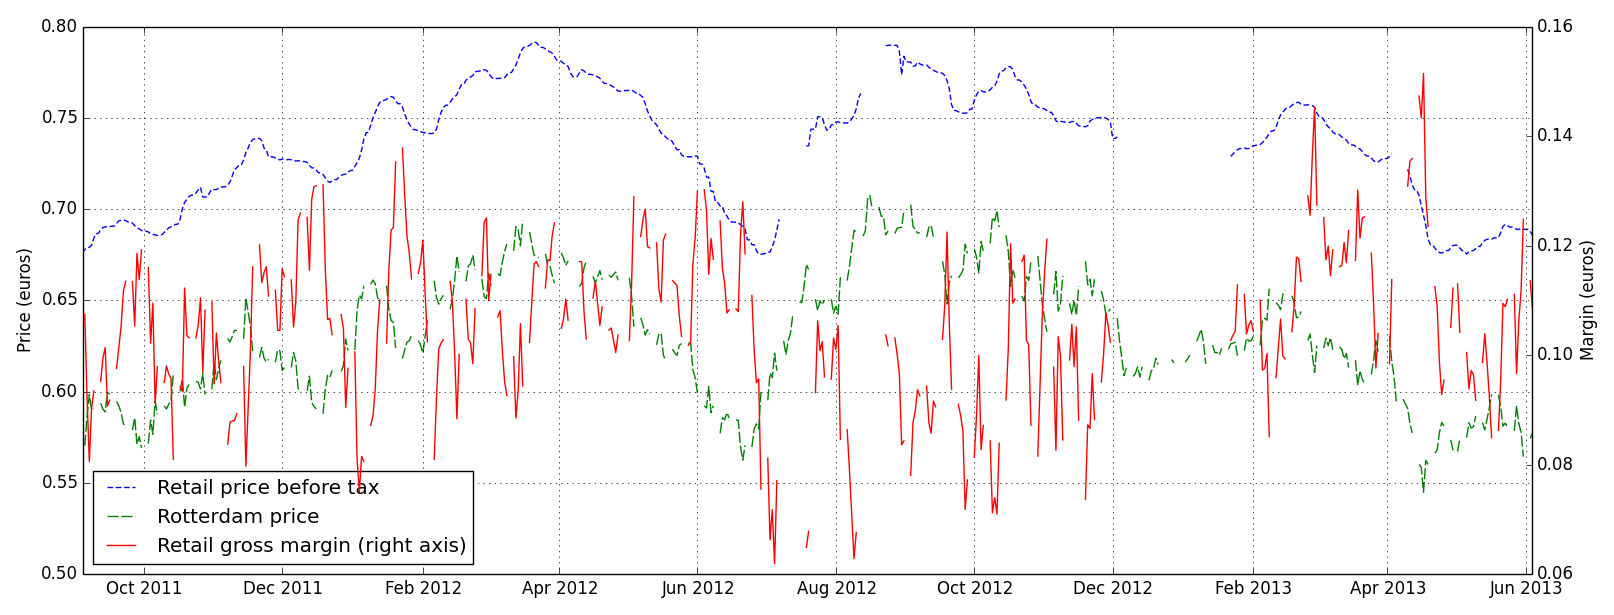
\includegraphics[width=16cm]{graphs/diesel_price_margin.png}
\end{figure}

\subsubsection{Price ridigity}

Data include prices at 9,932 gas stations in Mainland France, of which 421 are identified as highway gas stations and thus excluded from the analysis. Additionally, 381 stations are excluded due to apparent poor data quality (less than 10 prices observed or less than a price change per month). Overall, the number of prices retained in the analysis varies between 8,715 and 8,965 across days within the period studied. On average, c. 1,500 gas stations (c. 18\% of gas stations observed and retained) change prices within a day. The average gas station changes price a little less than every week.

\begin{figure}[!h]
    \caption{Daily number of price changes (09/2011-06/2012)}
	\centering
		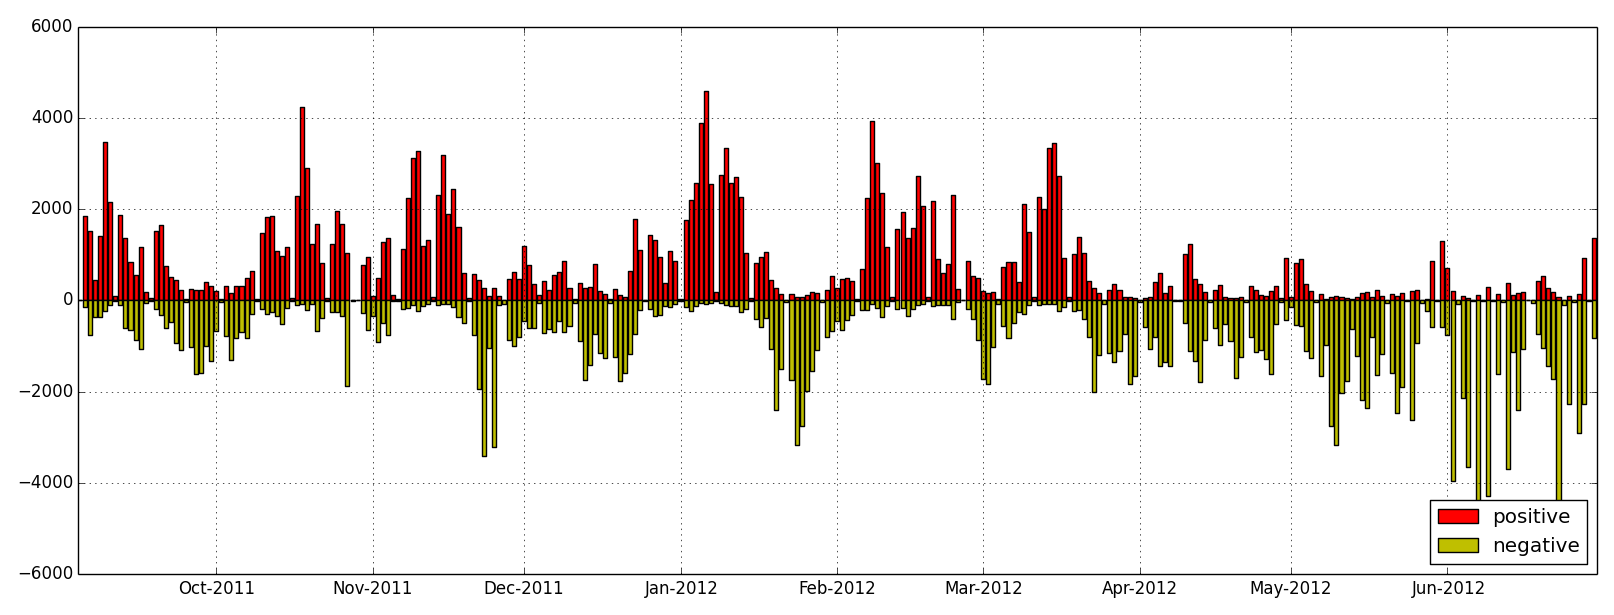
\includegraphics[width=16cm]{graphs/diesel_nb_price_chges.png}
    \floatfoot{The daily collection of prices has occasionally been delayed by a few hours resulting in some imprecision regarding the exact number of price changes occurring within one day}
\end{figure}

\subsubsection{Heterogeneity among gas stations}

Static price dispersion in French Data is easily seen in any single day price cross section. The resulting price distribution is bimodal, largely reflecting the presence of two dominant types of actors: supermarkets and oil companies. Supermarkets typically state that they use gasoline to attract customers, while oil companies mention the quality of the service to justify higher prices. Oil companies also traditionally enjoy more demand from businesses.

\section{Price dispersion vs. consumer information}

A simple way to measure temporal price dispersion between two stations with daily observations is to consider the probability that the station which is in general cheaper (in terms of day count) turns out to be more expensive. Formally, considering the prices $p_{it}$ and $p_{jt}$ of two stations $i$ and $j$ over $T_{ij}$ days, such that $p_{it} \ge p_{ij}$ is observed most of the time, the rank reversals statistic writes:

\begin{align*}
r_{ij} = \frac{1}{T_{ij}} \sum_{t=1}^{T_{ij}} \mathbbm{1}_{p_{jt} > p_{it}}
\end{align*}

A database is built in which observations are pairs of stations assumed to compete within the same market. In the following analysis, distance as the crow flies is used with an upper distance limit of 3km (robustness checks are joined in appendix). Rank reversals are thus computed for all gas stations in the database separated by a distance of less than 3km.

A sensitive issue in the empirical analysis is the treatment of differentiation, broadly understood as lasting differences in prices. Such an issue is traditionally addressed by working with price residuals (i.e. after taking out time and gas station fixed effects), which likely introduce errors in data. The analysis is thus performed with raw prices whenever differentiation is found to be relatively small, and with residual prices when differentiation requires it.

Finally, French data raise the issue of the nature of rank reversals measured by the statistic previously described. Indeed, the transformation by the firm "Total" of a significant number of its gas stations to low cost gas stations generates rank reversals which are clearly unrelated to the use of randomized pricing (cf. appendix). In order to avoid including "spurious rank reversals" in the analysis, the frequency of changes in price ranking was also considered in the analysis. Conservatively, pairs of gas stations involving such a brand and price policy change have been excluded from the analysis. It has also been checked that price policies implemented by competitors of rebranded gas stations were not significantly affected.

\begin{figure}[!h]
    \caption{Percentage of rank reversals among pairs}
	\centering
		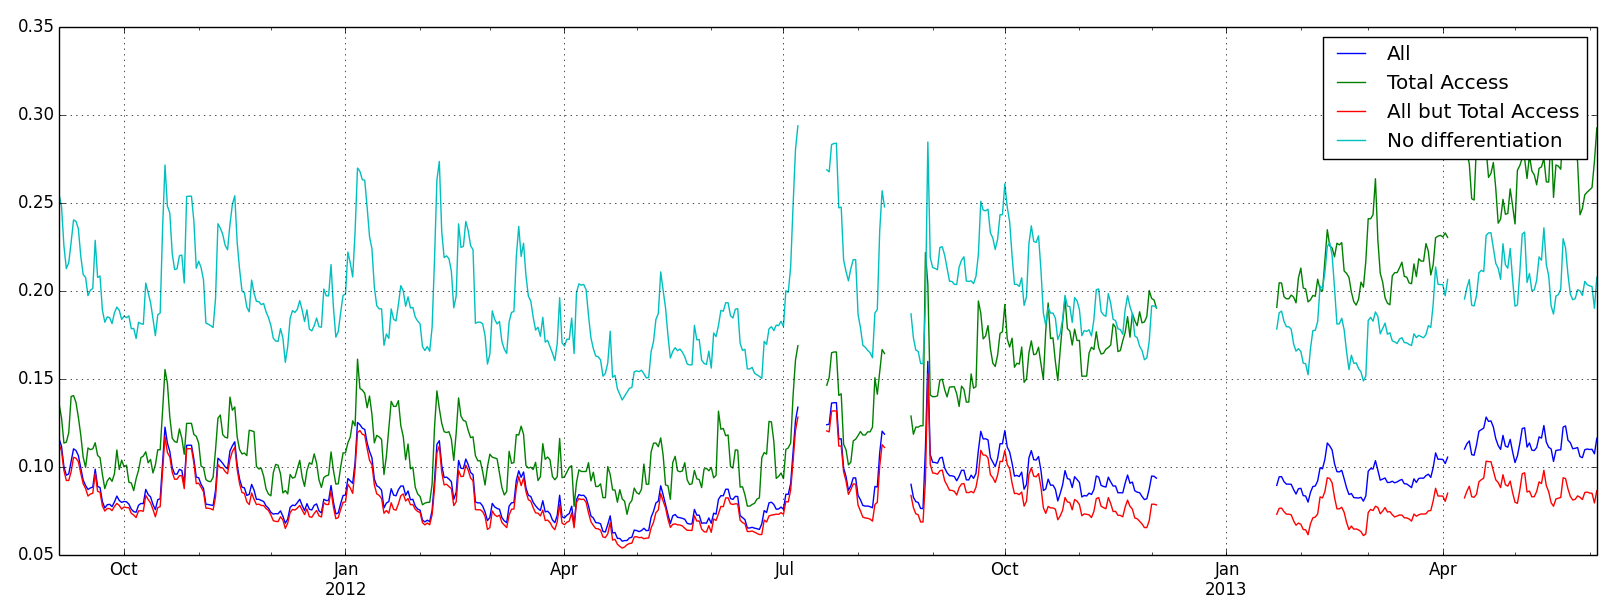
\includegraphics[width=16cm]{graphs/ecdf_rr_temporal.png}
    \floatfoot{Series represent for each day the percentage of pairs observed where the usual price order is not respected (reversed rank). No differentiation implies that pairs exhibit an average price difference below 2c/l.}
\end{figure}

Figure 3 displays the percentage of pairs of gas stations whose price rank is reversed on each day of the period studied. It illustrates how a naive use of rank reversals may lead to overestimate price dispersion ("All pairs" vs. "All but Total Access"). Among pairs of gas stations built with a maximum distance of 3km, the percentage of reversed pairs fluctuates between 5.4\% and 15.3\%  (mean 8.1\%). A large portion of pairs yet involve differentiated competitors (supermarkets are typically less expensive and thus always cheaper than most oil company gas stations). The "No differentiation" series results from a focus on pairs which exhibit an average price difference below 2c/l. Among these pairs, the minimum percentage of reversed pairs fluctuates between 13.8\% and 29.3\% (mean 19.5\%). From a consumer viewpoint, this translates in one chance in five to pay the highest price upon patronizing among two competitors of similar price level the one which is cheaper most of the time.

Using maximum 3km and 5km allows to build databases containing respectively 13,846 and 28,433 pairs of gas stations. As expected, rank reversals between two stations decreases in the average spread between their prices, with a large number exhibiting no rank reversals. In order to reduce the influence of static dispersion, the sample is subset based on the value of the average spread between prices. Results are presented for a maximum average spread of 0.02c/l i.e. a 1\% to 2\% average difference in prices.

\begin{table}
\caption{Pair rank reversals}
% {\renewcommand{\arraystretch}{0.8}
\centering
%\begin{center}
\begin{tabular}{lrrrrr}
\hline
{} & \multicolumn{3}{c}{Raw prices} & \multicolumn{2}{c}{Residual prices}  \\
{} & All & No Total & Price difference & Price difference & Price difference \\
{} & {} & Access & $\le$ 2c/l (mean) & $\le$ 2c/l (mean) & $\ge$ 2c/l (mean)\\
\hline
Max $d_{ij}$: 3km & {} & {} & {} & {} & {} \\
\hline
Nb pairs & 16,142 & 13,846 & 5,166 & 5,166 & 8,680 \\
Mean & 0.09 & 0.08 & 0.19 & 0.39 & 0.45 \\
Std & 0.13 & 0.12 & 0.13 & 0.11 & 0.05 \\
Median & 0.02 & 0.01 & 0.17 & 0.43 & 0.46 \\
\hline
Max $d_{ij}$: 5 km & {} & {} & {} & {} & {} \\
\hline
Nb pairs & 33,478 & 28,433 & 10,314 & 10,314 & 18,119 \\
Mean & 0.09 & 0.08 & 0.21 & 0.41 & 0.45 \\
Std & 0.13 & 0.12 & 0.13 & 0.10 & 0.04 \\
Median & 0.02 & 0.01 & 0.19 & 044 & 0.46 \\
\hline
\multicolumn{6}{l}{\small Pairs including a Total Access gas station are excluded in the three last columns}\\
\end{tabular}
%\end{center}
\end{table}

A clear ranking of empirical distribution functions of rank reversals can be observed among pairs of gas stations depending on distances. This is consistent with the idea that nearby gas stations compete in a (virtually) complete information setting, where there is no particular reason to expect rank reversals. Conversely, distance can create an information issue for other pairs, leading to the inexistence of an equilibrium in pure strategies.

\begin{figure}[H]
\centering
\caption{Empirical distribution functions of rank reversals (raw prices)}
\begin{subfigure}{.4\linewidth}
\centering
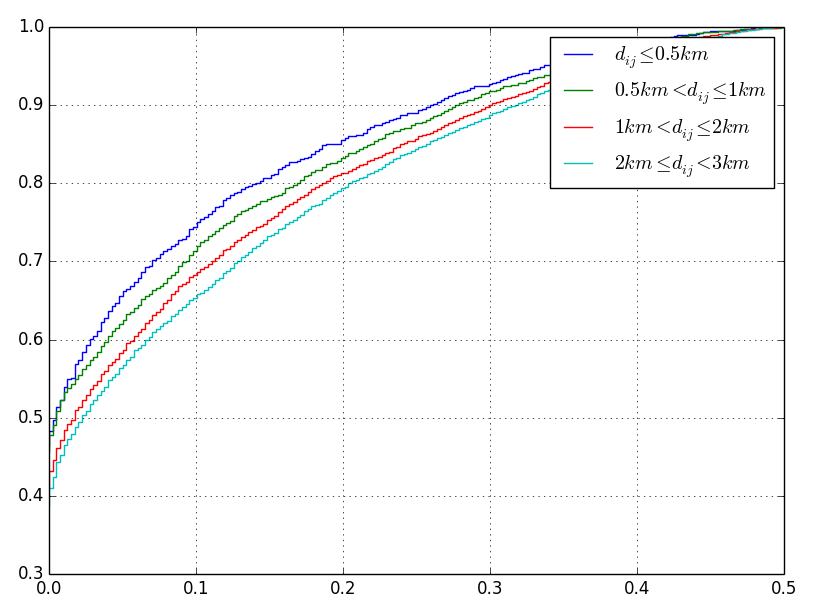
\includegraphics[width=6cm]{graphs/ecdf_rr_all.png}
\caption[short]{All pairs}
\end{subfigure}
\begin{subfigure}{.4\linewidth}
\centering
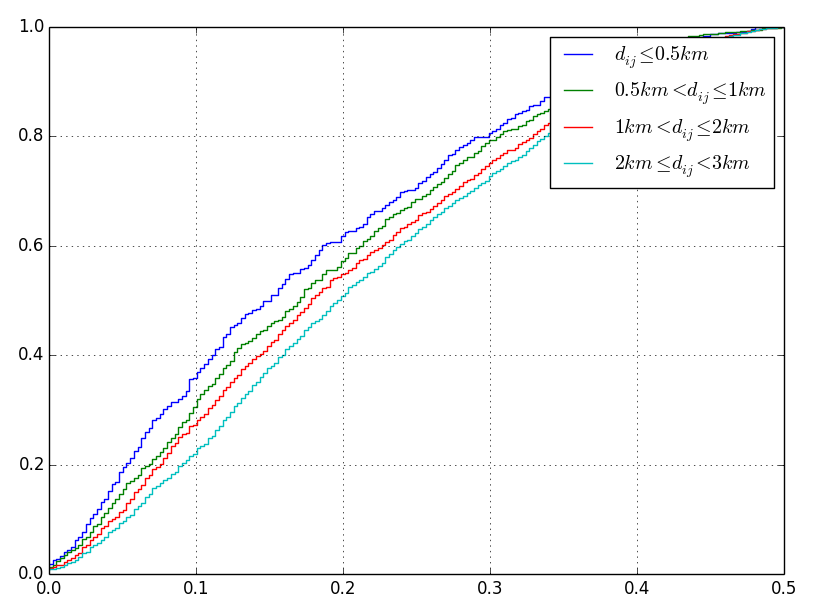
\includegraphics[width=6cm]{graphs/ecdf_rr_nodiff.png}
\caption[short]{Pairs with low differentiation}
\end{subfigure}
\end{figure}

In order to evaluate the hypothesis according to which information is connected to price dispersion, two measures of price dispersion: rank reversals and standard deviation in spread, are regressed on a proxy for consumer information: distance between stations.

\begin{table}[h]
\centering
\def\sym#1{\ifmmode^{#1}\else\(^{#1}\)\fi}
\caption{Regression of rank reversals}
\begin{tabular}{lccc}
\hline
\hline
{} & No differentiation & No differentiation & Differentiation \\
{} & raw prices & residual prices & residual prices \\
\hline
OLS: distance             &  0.014\sym{***}  &  0.020\sym{***}  &  0.001\sym{}\\
{}                        & (0.002)          & (0.002)          & (0.001)   \\
OLS: same corner                & -0.024\sym{***}  & -0.034\sym{***}  & -0.006\sym{***}\\
{}                        & (0.007)          & (0.006)          & (0.002) \\
Quantile 0.25: same corner      & -0.027\sym{***}  & -0.067\sym{***}  & -0.007\sym{***}\\
{}                        & (0.008)          & (0.010)          & (0.003)  \\
Quantile 0.50: same corner      & -0.024\sym{*}    & -0.030\sym{***}  & -0.007\sym{**}\\
{}                        & (0.011)          & (0.005)          & (0.002)    \\
Quantile 0.75: same corner      & -0.027\sym{*}    & -0.007\sym{*}    & -0.002\sym{}\\
{}                        & (0.014)          & (0.003)          & (0.001)   \\
\hline
N                         & 4,183            &   4,183          &     8,312    \\
\hline\hline
\multicolumn{4}{l}{\footnotesize Standard errors in parentheses}\\
\multicolumn{4}{l}{\footnotesize \sym{*} \(p<0.05\), \sym{**} \(p<0.01\), \sym{***} \(p<0.001\)}\\
\end{tabular}
\floatfoot{The "same corner" variable is a dummy variable that takes value one for pairs of gas stations separated by a distance of less than 500 meters, namely those for which consumers are expected to be relatively well informed about prices at each retailer.}\\
\end{table}

Overall, results seem to support the connection between price dispersion and consumer information. Pairs separated by a short distance exhibit less rank reversals, while the average price difference tends to be smaller. Though significant, the effect is weaker for differentiated gas stations. This might partly be due to errors introduced by the cleaning of prices. However, for pairs exhibiting little or no differentiation, results do not diffe significantly whether raw prices or residual prices are taken into account.

\section{Market price dispersion}

While the emphasis has so far been laid on examining empirical evidence about the link between price dispersion and consumer information, the following section seeks to compare predictions from a model a la \cite{VAR80} with French retail gasoline market data.

The methodology employed by \cite{TAP11} consists in considering each gas station successively as the center of a market delimited by a circle of a given radius (robustness of results to variations in radius size is checked). Various statistics accounting for price dispersion can then be computed for each market and period. If one observes $N$ stations close to each other (e.g. with a limit radius of 2km: if no two stations are separated by a distance of more than 2 km) and with prices posted over $T$ periods, this will result in $N*T$ observations as each station is successively considered and, for each station, a statistic representing price dispersion is computed at each period. An expected consequence is that it tends to over represent markets with higher gas station density (typically cities).

\begin{table}[h]
\caption{Overview of market price dispersion}
\begin{tabular}{lrrr}
\hline
{} & Radius 5km & Radius 3km & No overlap\\
\hline
Nb of markets & 6794 & 5614 & 386 \\
Avg nb competitors & 11.2 & 6.7 & 3.9 \\
\hline
Raw prices & & & \\
\hline
Market price range & 0.116 & 0.105 & 0.089\\
Market gain from search & 0.046 & 0.044 & 0.036 \\
Market price std & 0.046 & 0.045 & 0.045 \\
\hline
Residual prices & & & \\
\hline
Market price range & 0.033  & 0.028 & 0.020 \\
Market gain from search & 0.017 & 0.014 & 0.010 \\
Market price std & 0.011 & 0.011 & 0.010 \\
\hline
\end{tabular}
\floatfoot{Each statistic accounting for price dispersion is first computed for each local market across time. The table reports averages across markets. At the market level, price dispersion has been computed only for days when more than two thirds of competitors' prices were available. Only markets with more than 50 days of data are then taken into account to compute reported statistics.}
\end{table}


Regressions are then run using raw prices and cleaned prices. Also, in order to address the issue of overlapping markets, regression are performed on dispersion data generated in a way that prevents market overlap. Descriptive statistics performed on raw prices are provided.

Standard market dispersion statistics such as range and standard deviation are strongly influenced by static price dispersion. As a consequence, contrarily to the previous section where descriptives statistics performed on raw prices arguably provided a most conservative first idea of price dispersion, clean prices are now to be preferred despite their shortcomings. Results are reported with clean prices, raw prices for markets obtained with radiuses of respectively 3 and 5km. Additionnally, results are reported for non overlapping markets built in a way that is detailed in appendix.

\begin{table}[H]
%\renewcommand{\arraystretch}{0.7}
\def\sym#1{\ifmmode^{#1}\else\(^{#1}\)\fi}
\caption{Regressions of market dispersion}
\centering
\begin{tabular}{lcccc}
\hline
\hline
{} & All & All & No overlap & Stable markets\\
{} & Raw prices & Residual prices & Residual prices &  Residual prices \\
\hline
Gains from search & & & & \\
\hline
Nb competitors           &  0.003\sym{***}  &  0.001\sym{***}  &  0.001\sym{***}  & 0.001\sym{***} \\
{}                       & (0.000)          & (0.000)          & (0.000)          & (0.000)        \\
Cost                     &  0.007\sym{*  }  & -0.006\sym{*}    & -0.005\sym{}     & -0.005\sym{}   \\
{}                       & (0.003)          & (0.003)          & (0.003)          & (0.003)        \\
Intercept                &  0.015\sym{***}  &  0.015\sym{***}  & 0.013\sym{***}   &  0.012\sym{**} \\
{}                       & (0.004)          & (0.004)          & (0.004)          & (0.004)        \\
\hline
Standard deviation & & & & \\
\hline
Nb competitors           &  0.000\sym{***}  &  0.000\sym{***}  &  0.000\sym{***}  &  0.000\sym{}          \\
{}                       & (0.000)          & (0.000)          & (0.000)          & (0.000)    \\
Cost                     & -0.001\sym{   }  & -0.009\sym{***}  & -0.009\sym{***}  & -0.008\sym{***} \\
{}                       & (0.002)          & (0.002)          & (0.002)          & (0.003)         \\
Intercept                &  0.044\sym{***}  &  0.022\sym{***}  &  0.021\sym{***}  &  0.021\sym{***} \\
{}                       & (0.003)          & (0.003)          & (0.003)          & (0.004)    \\
\hline
Coefficient of variation & & & & \\
\hline
Nb competitors           &  0.000\sym{***}  &        \sym{}    &       \sym{}     &\\
{}                       & (0.000)          &                  &                  &\\
Cost                     & -0.024\sym{***}  &        \sym{}    &       \sym{}     &\\
{}                       & (0.001)          &                  &                  &\\
Intercept                &  0.064\sym{***}  &        \sym{}    &       \sym{}     &\\
{}                       & (0.002)          &                  &                  &\\
\hline
Range & & & & \\
\hline
Nb competitors           &  0.006\sym{***}  &  0.002\sym{***}  &  0.003\sym{***}  &  0.002\sym{***} \\
{}                       & (0.000)          & (0.000)          & (0.000)          & (0.000)         \\
Cost                     & -0.004\sym{}     & -0.025\sym{***}  & -0.021\sym{***}  & -0.019\sym{***} \\
{}                       & (0.005)          & (0.005)          & (0.005)          & (0.006)         \\
Intercept                &  0.074\sym{***}  & 0.048\sym{***}   &  0.041\sym{***}  &  0.038\sym{***} \\
{}                       & (0.007)          & (0.007)          & (0.007)          & (0.008)         \\
\hline
N                        & 2,756,096        & 2,756,096        & 493,356          &\\
\hline\hline
\multicolumn{4}{l}{\footnotesize Standard errors in parentheses}\\
\multicolumn{4}{l}{\footnotesize \sym{*} \(p<0.05\), \sym{**} \(p<0.01\), \sym{***} \(p<0.001\)}\\
\end{tabular}
\end{table}

Estimation results show that dispersion is increasing in the number of firm and decreasing in price.

\section{Conclusion}

This paper discusses the methodology of \cite{TAP11} to measure price dispersion in the field and see how it compares with potential theoretical explanations. The presence of differentiation in the French retail gasoline market yet requires to work both with raw and residual prices.

Rank reversals are generally found to be less frequent for pairs gas stations separated by a short distance i.e. competitors whose prices are easy to compare for consumers, hence supporting the connection between consumer information and price dispersion. When differentiation is significant, regressions performed on residual prices show a weaker effect of distance. This suggests that one should be cautious when there is differentiation despite the high number of rank reversals that one obtains with residual prices.

At the market level, price dispersion is found to increase with the number of competitors, and decrease with cost. This is consistant with predictions of a model a la \cite{VAR80}. Importantly, in the presence of significant differentiation, working with raw prices typically leads to overestimate price dispersion reflecting randomized pricing. The average gain from search across markets and time over the period computed with residual prices varies between 1.7 and 1.0 Euro cents per litre meaning that knowing all prices in the market allows to spare on average between 50 and 85 Euro cents for a gas tank of 50L.

Further research remains to be undertaken in two directions: one is the investigation of the heterogeneity in local market price patterns and the other is the combined analysis of price dispersion together with data about consumer search (e.g. price comparison website frequentation over time if data are released).

\newpage

\bibliography{references}

\newpage

\appendix

\section{Spurious rank reversals}

The following figure displays prices posted at a gas station which is rebranded "Total Access" (low cost brand of Total) in the middle of the period studied and at two nearby gas stations. It is easily seen how naively considering the percentage of rank reversals of the rebranded gas station vs. each of its competitors over the whole period would lead to record spurious price dispersion. The price level indeed changes abruptly in a way that cannot go unnoticed by consumers. It thus clearly does not reflect any used of randomized pricing and such rank reversals are thus excluded from the analysis. More generally, this suggests the need to control the frequency of changes in price ranking so as to limit the risk of capturing dispersion reflecting such deterministic changes in pricing policies.

\ \\
\begin{figure}[H]
    \caption{Prices of three stations in Chalons-en-Champagne}
	\centering
		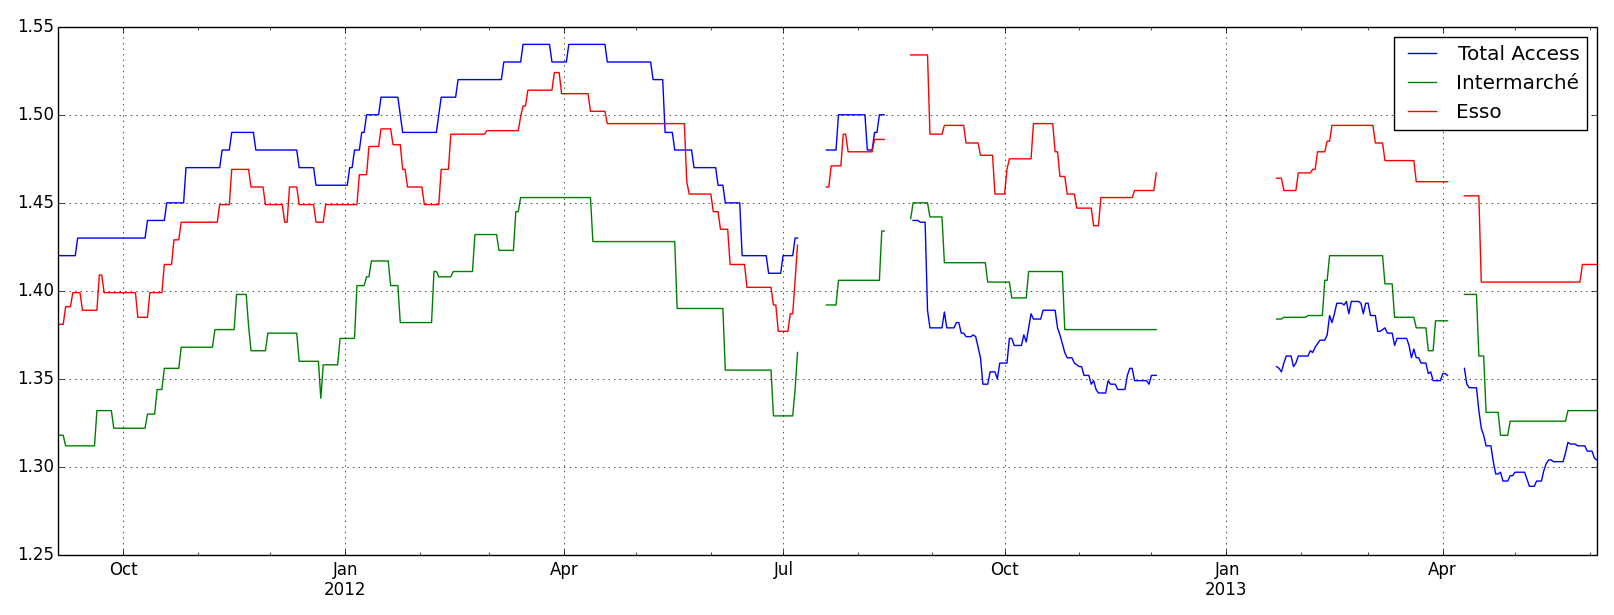
\includegraphics[width=16cm]{graphs/spurious_total_access_rr.png}
	\floatfoot{}
\end{figure}

\newpage

\section{Additionnal regression results}

\begin{table}[!htbp]\centering
\def\sym#1{\ifmmode^{#1}\else\(^{#1}\)\fi}
\caption{Regression of standard deviation in spread}
\begin{tabular}{lrrr}
\hline
\hline
{} & No differentiation & No differentiation & Differentiation \\
{} & raw prices & residual prices & residual prices \\
\hline
OLS: distance &  0.001 \sym{***}&      0.001\sym{***}&       0.000\sym{***}\\
{} &     (0.000)         &     (0.000)         &     (0.000)   \\
OLS: dummy &  -0.001\sym{***}&      -0.001\sym{***}&     -0.001\sym{***}\\
{} &    (0.000)     &     (0.000)         &     (0.000) \\
Quantile 0.25: dummy     &       -0.001\sym{**}&       -0.001\sym{**}&       -0.000\sym{}\\
{} &     (0.000)       &     (0.000)         &     (0.000)  \\
Quantile 0.50: dummy     &       -0.001\sym{**}&      -0.001\sym{*}&       -0.000\sym{}\\
{} &  (0.000)         &     (0.000)         &     (0.000)    \\
Quantile 0.75: dummy     &       -0.001\sym{**}&     -0.001\sym{**}&       -0.000\sym{}\\
{} &     (0.001)         &     (0.001)         &     (0.000)   \\
\hline
N      &     4,183         &     4,183      &     8,312    \\
\hline\hline
\multicolumn{4}{l}{\footnotesize Standard errors in parentheses}\\
\multicolumn{4}{l}{\footnotesize \sym{*} \(p<0.05\), \sym{**} \(p<0.01\), \sym{***} \(p<0.001\)}\\
\end{tabular}
\end{table}

\section{In progress}

\subsection{Number of digits after decimal point}

There is heterogeneity between the number of digits displayed after decimal point among stations. Some stations indeed appear to restrict themselves to two digits after decimal point, hence giving up the possibility to undercut or match a competitor's price. Though accounting for this phenomenon is out of the scope of this paper, its connection with price dispersion is (to be) investigated.

\subsection{Leadership}

Maskin and Tirole (1988) [TODO: add ref] offer an alternative explanation for rank reversals. They indeed show that in a context where sellers have to commit on prices for at least one period, cycles can occur which are characterized by periods of undercutting punctuated by one firm accepting to set a high price when margin becomes too small. XXX [TODO: add ref] find evidence of such cycles with XXX data. Though standard test rule out the presence such cycles in French data, evidence of other specific patterns of prices has been found.

\subsection{Monopoly, information, inventory and rule of thumb}

Finally, a natural explanation for rank reversals could be that gas stations actually do not really compete and that their prices simply reflect their flow of information and/or inventory through more or less complex pricing rules. Such explanations are (to be) examined.

\end{document} 